%% Run LaTeX on this file several times to get Table of Contents,
%% cross-references, and citations.
\documentclass[11pt]{book}
\usepackage{gvv-book}
\usepackage{gvv}
\usepackage[sectionbib,authoryear]{natbib}% for name-date citation comment the below line
\setcounter{secnumdepth}{3}
\setcounter{tocdepth}{2}

\makeindex

\begin{document}

\frontmatter

\booktitle{GEOMETRY}

\subtitle{Through Algebra}

\AuAff{Chakali Suresh}

\titlepage

\tableofcontents

\setcounter{page}{0}

\mainmatter

\chapter{Triangle}
Consider a triangle with vertices
\begin{align}
\vec{A} = \myvec{0 \\ -5},\,
\vec{B} = \myvec{-2 \\ -4},\,
\vec{C} = \myvec{-5 \\ -4}
\end{align}

\section{Median}
\begin{enumerate}[label=\thesection.\arabic*.,ref=\thesection.\theenumi]
\numberwithin{equation}{enumi}

%Question 1.2.1:
\item if $\vec{D}$ divides $BC$ in the ratio of $k : 1$,
        \begin{align}
                \vec{D} &= \frac{k\vec{C} + \vec{B}}{K+1}
        \end{align}
        Find the mid points $\vec{D}, \vec{E}, \vec{F}$ of the sides $AB,BC$ and $CA$ respectively.\\
        \solution\\
        Since $\vec{D}$ is the midpoint of $BC$
        \begin{align}
                \text{Let} k &= 1\\
                \therefore \text{we get }\\
                \implies \vec{D} &= \frac{\vec{C} + \vec{B}}{2}\\
                &= \frac{1}{2} \times \myvec{-5 \\ -4} + \myvec{-2 \\ -4}\\
                &= \frac{1}{2} \myvec{-7 \\ -8}
        \end{align}

        Similarly,
        \begin{align}
                \implies \vec{E} &= \frac{\vec{A} + \vec{C}}{2}\\
                &= \frac{1}{2} \myvec{-5 \\ -9}\\
                \implies \vec{F} &= \frac{\vec{A} + \vec{B}}{2}\\
                &= \frac{1}{2} \myvec{-2 \\ -9}
        \end{align}
		\begin{figure}[H]
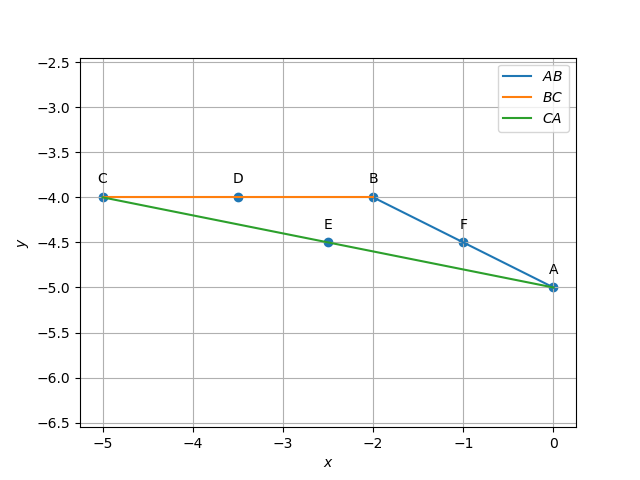
\includegraphics [width=\columnwidth] {/sdcard/Documents/figs/Midpoint}
        \caption{  Triangle $\vec{ABC}$ with midpoints $\vec{D,E,F}$}
\label{fig:Triangle ABC}
\end{figure}

%Question 1.2.2:
        \item Find the equations of $AD, BE$ and $CF$.
        \solution:\\
        Given, 
        \begin{align}
        \vec{D} &= \myvec{\frac{-7}{2} \\ -4}\\
        \vec{E} &= \myvec{\frac{-5}{2} \\ \frac{-9}{2}}\\
        \vec{F} &= \myvec{-1 \\ \frac{-9}{2}}
        \end{align}
        \begin{enumerate}
       \item The normal equation for the median AD is
        \begin{align}
        \vec{n}^{\top}\myvec{\vec{x}-\vec{A}} &= 0\\
         \therefore \vec{n}^{\top}\vec{x} &=  \vec{n}^{\top}\vec{A}
        \end{align}
\begin{align}
	\vec{m} &= \vec{D}- \vec{A} \\
&=\myvec{\frac{-7}{2}\\ -4} - \myvec{0 \\ -5}
	 =\myvec{\frac{-7}{2} \\ 1}\\
 	\implies  \vec{n} &=\myvec{0 & 1 \\ -1 & 0} \vec{m}\\
  &= \myvec{0 & 1 \\ -1 & 0} \myvec{\frac{-7}{2}\\ 1}\\
  &= \myvec{1 \\ \frac{7}{2}}\\
  \therefore \vec{n}^{\top} &= \myvec{1 & \frac{7}{2}}
\end{align}
Hence the normal equation of median $AD$ is 
\begin{align}
\vec{n}^{\top}\vec{x} &= \vec{n}^{\top}\vec{A}\\
\implies \myvec{1 & \frac{7}{2}}\vec{x} &= \myvec{1 & \frac{7}{2}}\myvec{0\\-5}\\
   \myvec{1 & \frac{7}{2}}\vec{x} &= -\frac{35}{2}\\
	\myvec{2 & 7}\vec{x} &= -35
\end{align}

\item The normal equation for the median $BE$ is
        \begin{align}
        \vec{n}^{\top}\myvec{\vec{x}-\vec{B}} &= 0\\
         \therefore \vec{n}^{\top}\vec{x} &=  \vec{n}^{\top}\vec{B}
        \end{align}
\begin{align}
	\vec{m} &= \vec{E}- \vec{B} \\
&=\myvec{\frac{-5}{2}\\ \frac{-9}{2}} - \myvec{-2 \\ -4}
	 =\myvec{\frac{-1}{2} \\ \frac{-1}{2}}\\
 	\implies  \vec{n} &=\myvec{0 & 1 \\ -1 & 0} \vec{m}\\
  &= \myvec{0 & 1 \\ -1 & 0} \myvec{\frac{-1}{2}\\ \frac{-1}{2}}\\
  &= \myvec{\frac{-1}{2} \\ \frac{1}{2}}\\
  \therefore \vec{n}^{\top} &= \myvec{\frac{-1}{2} & \frac{1}{2}}
\end{align}
Hence the normal equation of median $BE$ is 
\begin{align}
\vec{n}^{\top}\vec{x} &= \vec{n}^{\top}\vec{B}\\
\implies \myvec{\frac{-1}{2} & \frac{1}{2}}\vec{x} &= \myvec{\frac{-1}{2} & \frac{1}{2}}\myvec{-2\\-4}\\
   \myvec{\frac{-1}{2} & \frac{1}{2}}\vec{x} &= -1\\
	\myvec{-1 & 1}\vec{x} &= -2
\end{align}

\item The normal equation for the median $CF$ is
        \begin{align}
        \vec{n}^{\top}\myvec{\vec{x}-\vec{C}} &= 0\\
         \therefore \vec{n}^{\top}\vec{x} &=  \vec{n}^{\top}\vec{C}
        \end{align}
\begin{align}
	\vec{m} = \vec{F}- \vec{C}
&=\myvec{-1 \\ \frac{-9}{2}} - \myvec{-5 \\ -4}
	 =\myvec{4 \\ \frac{-1}{2}}\\
 	\implies  \vec{n} &=\myvec{0 & 1 \\ -1 & 0} \vec{m}\\
  &= \myvec{0 & 1 \\ -1 & 0} \myvec{4 \\ \frac{-1}{2}}\\
  &= \myvec{\frac{-1}{2} \\ -4}\\
  \therefore \vec{n}^{\top} &= \myvec{\frac{-1}{2} & -4}
\end{align}
Hence the normal equation of median $CF$ is 
\begin{align}
\vec{n}^{\top}\vec{x} &= \vec{n}^{\top}\vec{C}\\
\implies \myvec{\frac{-1}{2} & -4}\vec{x} &= \myvec{\frac{-1}{2} & -4}\myvec{-5\\-4}\\
   \myvec{\frac{-1}{2} & -4}\vec{x} &= \frac{37}{2}\\
	\myvec{-1 & -8}\vec{x} &= 37
\end{align}
\end{enumerate}
		\begin{figure}[H]
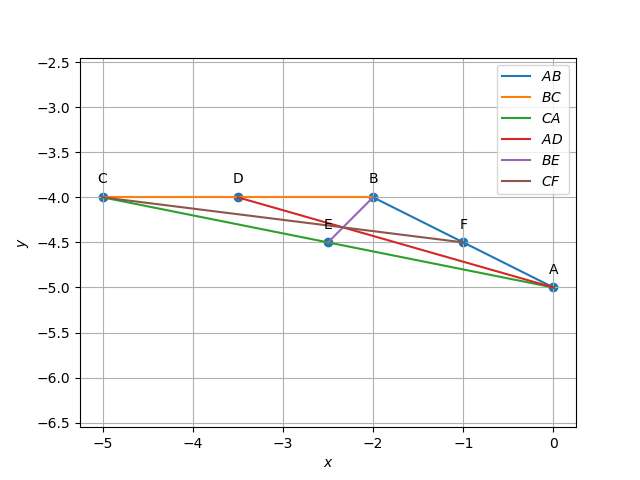
\includegraphics [width=\columnwidth] {/sdcard/Documents/figs/Median}
			\caption{Triangle $ABC$ with medians $AD, BE, CF$}
\label{fig:Median point}
\end{figure}

%Question 1.2.3:
	\item Find the intersection $\vec{G}$ of $BE$ and $CF$.\\
\solution \\
The equations of $BE$ is,
\begin{align}
   \myvec{-1 & 1}\vec{x} &= -2
\label{eq:1.2.3,1}
\end{align}
The equations of $CF$ is,
\begin{align}
   \myvec{-1 & -8}\vec{x} &= 37
\label{eq:1.2.3,2}
\end{align}
From \eqref{eq:1.2.3,1} and \eqref{eq:1.2.3,2} the augmented matrix is
\begin{align}
    \label{eq:matrowoperations}
    \myvec{-1 & 1 & -2
    \\
    -1 & -8 & 37
    }
     \xleftrightarrow[]{R_1 \leftarrow R_1 \times -1}
    \myvec{
    1 & -1 & 2
    \\
    -1 & -8 & 37 
    }
    \\
     \xleftrightarrow[]{R_2\leftarrow R_2+R_1}
    \myvec{
    1 & -1 & 2
    \\
    0 & -9 & 39 
    }\\
     \xleftrightarrow[]{R_2\leftarrow R_2 \times -1/9}
    \myvec{
    1 & -1 & 2
    \\
    0 & 1 & \frac{-13}{3}
    }
    \\
     \xleftrightarrow[]{R_1\leftarrow R_1+R_2}
    \myvec{
    1 & 0 & \frac{-7}{3}
    \\
    0 & 1 & \frac{-13}{3}
    }
\end{align} 
using Gauss elimination.  Therefore, 
\begin{align}
\vec{G} = \myvec{\frac{-7}{3} \\ \frac{-13}{3}}
\end{align}
		\begin{figure}[H]
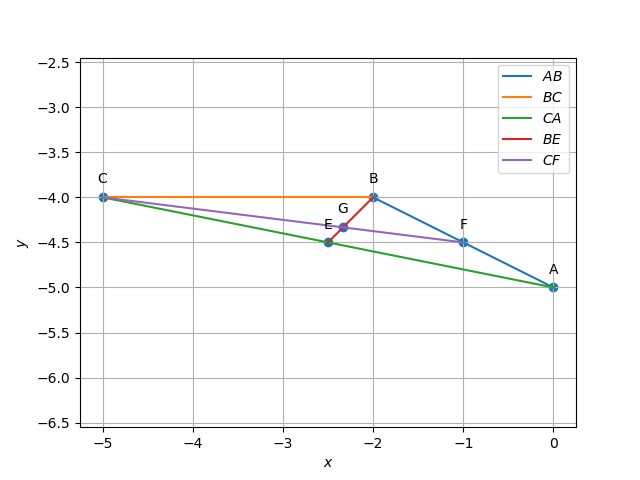
\includegraphics [width=\columnwidth] {/sdcard/Documents/figs/Centroid}
			\caption{Centroid$\vec{(G)}$ of triangle $ABC$}
\label{fig:Triangle ABC}
\end{figure}

%Question 1.2.4: 
\item Verify that 
		\begin{align}
			\frac{BG}{GE} = 
			\frac{CG}{GF} =
			\frac{AG}{GD} =2 
		\end{align}
 \solution\\ In order to verify the above equation we first need to find $\vec{G}$.$\vec{G}$ is the intersection of $BE$ and $CF$,Using the value of $\vec{G}$ from (1.2.3).
\begin{align}
		\vec{G} = \myvec{\frac{-7}{3} \\ \frac{-13}{3}}
\end{align}
Also,We know that $\vec{A,B,C,D,E}$ and $\vec{F}$ are midpoints of $BC, CA$ and $AB$ respectively from (1.2.1).
\begin{align}
        \vec{A} &= \myvec{0 \\ -5}, \vec{B} = \myvec{-2 \\ -4}, \vec{C} = \myvec{-5 \\ -4}\\
		\vec{D} &= \myvec{\frac{-7}{2} \\ -4},
		\vec{E} = \myvec{\frac{-5}{2} \\ \frac{-9}{2}},
		\vec{F} = \myvec{-1 \\ \frac{-9}{2}}
\end{align}
\begin{enumerate}
\item Calculating the ratio of $BG$ and $GE$,
\begin{align}
		\label{eq:tri-pts/1} \vec{G}-\vec{B} &= \myvec{\frac{-1}{3} \\ \frac{-1}{3}} \\
		\label{eq:tri-pts/2} \vec{E}-\vec{G} &= \myvec{\frac{-1}{6} \\ \frac{-1}{6}} \\
		\label{eq:tri-pts/3} \norm{\vec{G}-\vec{B}} &= \sqrt{\brak{\frac{-1}{3}}^2 + \brak{\frac{-1}{3}}^{2}} &= \frac{\sqrt{2}}{3} \\
		\label{eq:tri-pts/4} \norm{\vec{E}-\vec{G}} &= \sqrt{\brak{\frac{-1}{6}}^2 + \brak{\frac{-1}{6}}^2} &= \frac{\sqrt{2}}{6} \\
	\label{eq:tri-pts/5} \frac{BG}{GE} &= \frac{\norm{\vec{G}-\vec{B}}}{\norm{\vec{E}-\vec{G}}} &= \frac{\frac{\sqrt{2}}{3}}{\frac{\sqrt{2}}{6}} &= 2  
\end{align}		

\item Calculating the ratio of $CG$ and $GF$,
\begin{align}
		\label{eq:tri-pts/6} \vec{G}-\vec{C} &= \myvec{\frac{8}{3} \\ \frac{-1}{3}} \\
		\label{eq:tri-pts/7} \vec{F}-\vec{G} &= \myvec{\frac{4}{3} \\ \frac{-1}{6}} \\
		\label{eq:tri-pts/8} \norm{\vec{G}-\vec{C}} &= \sqrt{\brak{\frac{8}{3}}^2 + \brak{\frac{-1}{3}}^{2}} &= \frac{\sqrt{65}}{3} \\
		\label{eq:tri-pts/9} \norm{\vec{F}-\vec{G}} &= \sqrt{\brak{\frac{4}{3}}^2 + \brak{\frac{-1}{6}}^2} &= \frac{\sqrt{65}}{6} \\
	  \label{eq:tri-pts/10} \frac{CG}{GF} &= \frac{\norm{\vec{G}-\vec{C}}}{\norm{\vec{F}-\vec{G}}} &= \frac{\frac{\sqrt{65}}{3}}{\frac{\sqrt{65}}{6}} &= 2  
\end{align}		

\item Calculating the ratio of $AG$ and $GD$,
\begin{align}
		\label{eq:tri-pts/11} \vec{G}-\vec{A} &= \myvec{\frac{-7}{3} \\ \frac{2}{3}} \\
		\label{eq:tri-pts/12} \vec{D}-\vec{G} &= \myvec{\frac{-7}{6} \\ \frac{1}{3}} \\
		\label{eq:tri-pts/13} \norm{\vec{G}-\vec{A}} &= \sqrt{\brak{\frac{-7}{3}}^2 + \brak{\frac{2}{3}}^{2}} &= \frac{\sqrt{53}}{3} \\
		\label{eq:tri-pts/14} \norm{\vec{D}-\vec{G}} &= \sqrt{\brak{\frac{-7}{6}}^2 + \brak{\frac{1}{3}}^2} &= \frac{\sqrt{53}}{6} \\
	\label{eq:tri-pts/15} \frac{AG}{GD} &= \frac{\norm{\vec{G}-\vec{A}}}{\norm{\vec{D}-\vec{G}}} &= \frac{\frac{\sqrt{53}}{3}}{\frac{\sqrt{53}}{6}} &= 2  
\end{align}		
\end{enumerate}

From \eqref{eq:tri-pts/5}, \eqref{eq:tri-pts/10}, \eqref{eq:tri-pts/15}
\begin{align}
		\frac{BG}{GE} = 
		\frac{CG}{GF} =
		\frac{AG}{GD} = 2
\end{align}

%Question 1.2.5: 
\item Show that $\vec{A}, \vec{G}$ and $\vec{D}$ are collinear.\\
\solution 
Given that,
\begin{align}
    \vec{A} = \myvec{0\\-5}
\end{align}
We need to show that points $\vec{A},\vec{D},\vec{G}$ are collinear.
From Problem 1.2.3 We know that, The point $\vec{G}$ is 
\begin{align}
    \vec{G} &=\myvec{\frac{-7}{3}\\ \frac{-13}{3}}
\end{align}
And from Problem 1.2.1 We know that, The point $\vec{D}$ is 
\begin{align}
    \vec{D} &=\myvec{\frac{-7}{2}\\ 4}
\end{align}
In Problem 1.1.3, There is a theorem/law mentioned i.e.,

Points $\vec{A},\vec{D},\vec{G}$ are defined to be collinear if 
\begin{align}
    \text{rank}\myvec{
    1 & 1 & 1\\
    \vec{A} & \vec{D} & \vec{G} \\
    } &= 2 
\end{align} 
Using the above law/Theorem Let
\begin{align}
    \vec{R}&=\myvec{
    1 & 1 & 1
    \\
    0 & \frac{-7}{2} & \frac{-7}{3}
    \\
    -5 & 4 & \frac{-13}{3}
    } 
\end{align} 
The matrix $\vec{R}$ can be row reduced as follows,
\begin{align}
    \label{eq:mat_row_operations}
    \myvec{
    1 & 1 & 1
    \\
    0 & \frac{-7}{2} & \frac{-7}{3}
    \\
    -5 & 4 & \frac{-13}{3}
    } 
     \xleftrightarrow[]{R_3 \leftarrow R_3+5R_1}
    \myvec{
    1 & 1 & 1
    \\
    0 & \frac{-7}{2} & \frac{-7}{3}
    \\
    0 & 1 & \frac{2}{3} 
    }
    \\
     \xleftrightarrow[]{R_2\leftarrow \frac{-7}{2}R_2}
    \myvec{
    1 & 1 & 1
    \\
    0 & 1 & \frac{2}{3}
    \\
    0 & 1 &  \frac{2}{3}
    }
    \\
     \xleftrightarrow[]{R_3\leftarrow R_3-R_2}
    \myvec{
    1 & 1 & 1
    \\
    0 & 1 & \frac{2}{3}
    \\
    0 & 0 & 0
    }
\end{align}
Rank of above matrix is 2.\\
Hence, we proved that that points $\vec{A},\vec{D},\vec{G}$ are collinear.

%Question 1.2.6: 
\item Verify that 
		\begin{align}
			\vec{G}=\frac{\vec{A}+\vec{B}+\vec{C}}{3}
		\end{align}
$\vec{G}$ is known as the {\em centroid} of $\triangle ABC$.\\
\solution\\
\begin{align}
 \vec{G}=\frac{\vec{A}+\vec{B}+\vec{C}}{3}   
\end{align}
let us first evaluate the R.H.S of the equation
\begin{equation}
\begin{split}
\label{eq:centroid}
    \vec{G}&= \frac{\myvec{0\\-5}+\myvec{-2\\-4}+\myvec{-5\\-4}}{3}\\    
    &= \myvec{\frac{0-2-5}{3} \\ \frac{-5-4-4}{3}}\\
     &= \myvec{\frac{-7}{3}\\ \frac{-13}{3}}
\end{split}
\end{equation}
Hence verified.

%Question 1.2.7: 
\item Verify that 
		\begin{align}
\vec{A}-\vec{F}=\vec{E}-\vec{D}
		\end{align}
The quadrilateral $AFDE$ is defined to be a parallelogram.\\
\solution \\
Given that,
\begin{align}
    \vec{A} = \myvec{0\\-5}
    \quad
    \vec{B} &= \myvec{-2\\-4}
    \quad
    \vec{C} = \myvec{-5\\-4}\\
    \vec{D} = \myvec{\frac{-7}{2}\\ -4 }
    \quad
    \vec{E} &= \myvec{\frac{-5}{2}\\ \frac{-9}{2}}
    \quad
    \vec{F} = \myvec{-1\\ \frac{-9}{2}}
\end{align}
Evaluating the L.H.S of the equation
\begin{align}
    \vec{A}-\vec{F}&=\myvec{0\\-5}-\myvec{-1\\ \frac{-9}{2} }\\
    &=\myvec{ -1 \\ \frac{-1}{2} }
\end{align} 
Evaluating the R.H.S of the equation
\begin{align}
    \vec{E}-\vec{D}&=\myvec{\frac{-5}{2}\\ \frac{-9}{2}}-\myvec{\frac{-7}{2}\\ -4 }\\
    &=\myvec{-1 \\ \frac{-1}{2} }
\end{align}
Hence verified that, R.H.S = L.H.S
\begin{align}
	\vec{A}-\vec{F} = \vec{E}-\vec{D}
\end{align}
\begin{figure}[H]
	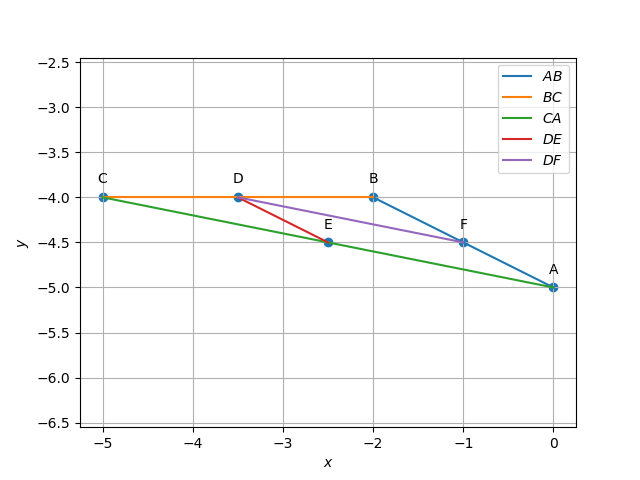
\includegraphics[width=\columnwidth]{/sdcard/Documents/figs/Parallelogram}
	\caption{$AFDE$ form a parallelogram in triangle ABC}
	\label{fig:Parallelogram}
\end{figure}

\latexprintindex
\end{enumerate}
\end{document}

 
